\section{Main Processor}

The main processor is in charge of generating the sequencer signals for reading the detector, configuring integrated circuits, monitoring interlocks, and communicating via Ethernet protocol. As main processor we selected the Trenz Electronic TE0720-04-62I33MA SoC-Module. \autoref{fig:soc} shows TE0720-04-62I33MA SoC-Module.

\begin{figure}[ht]
  \centering
  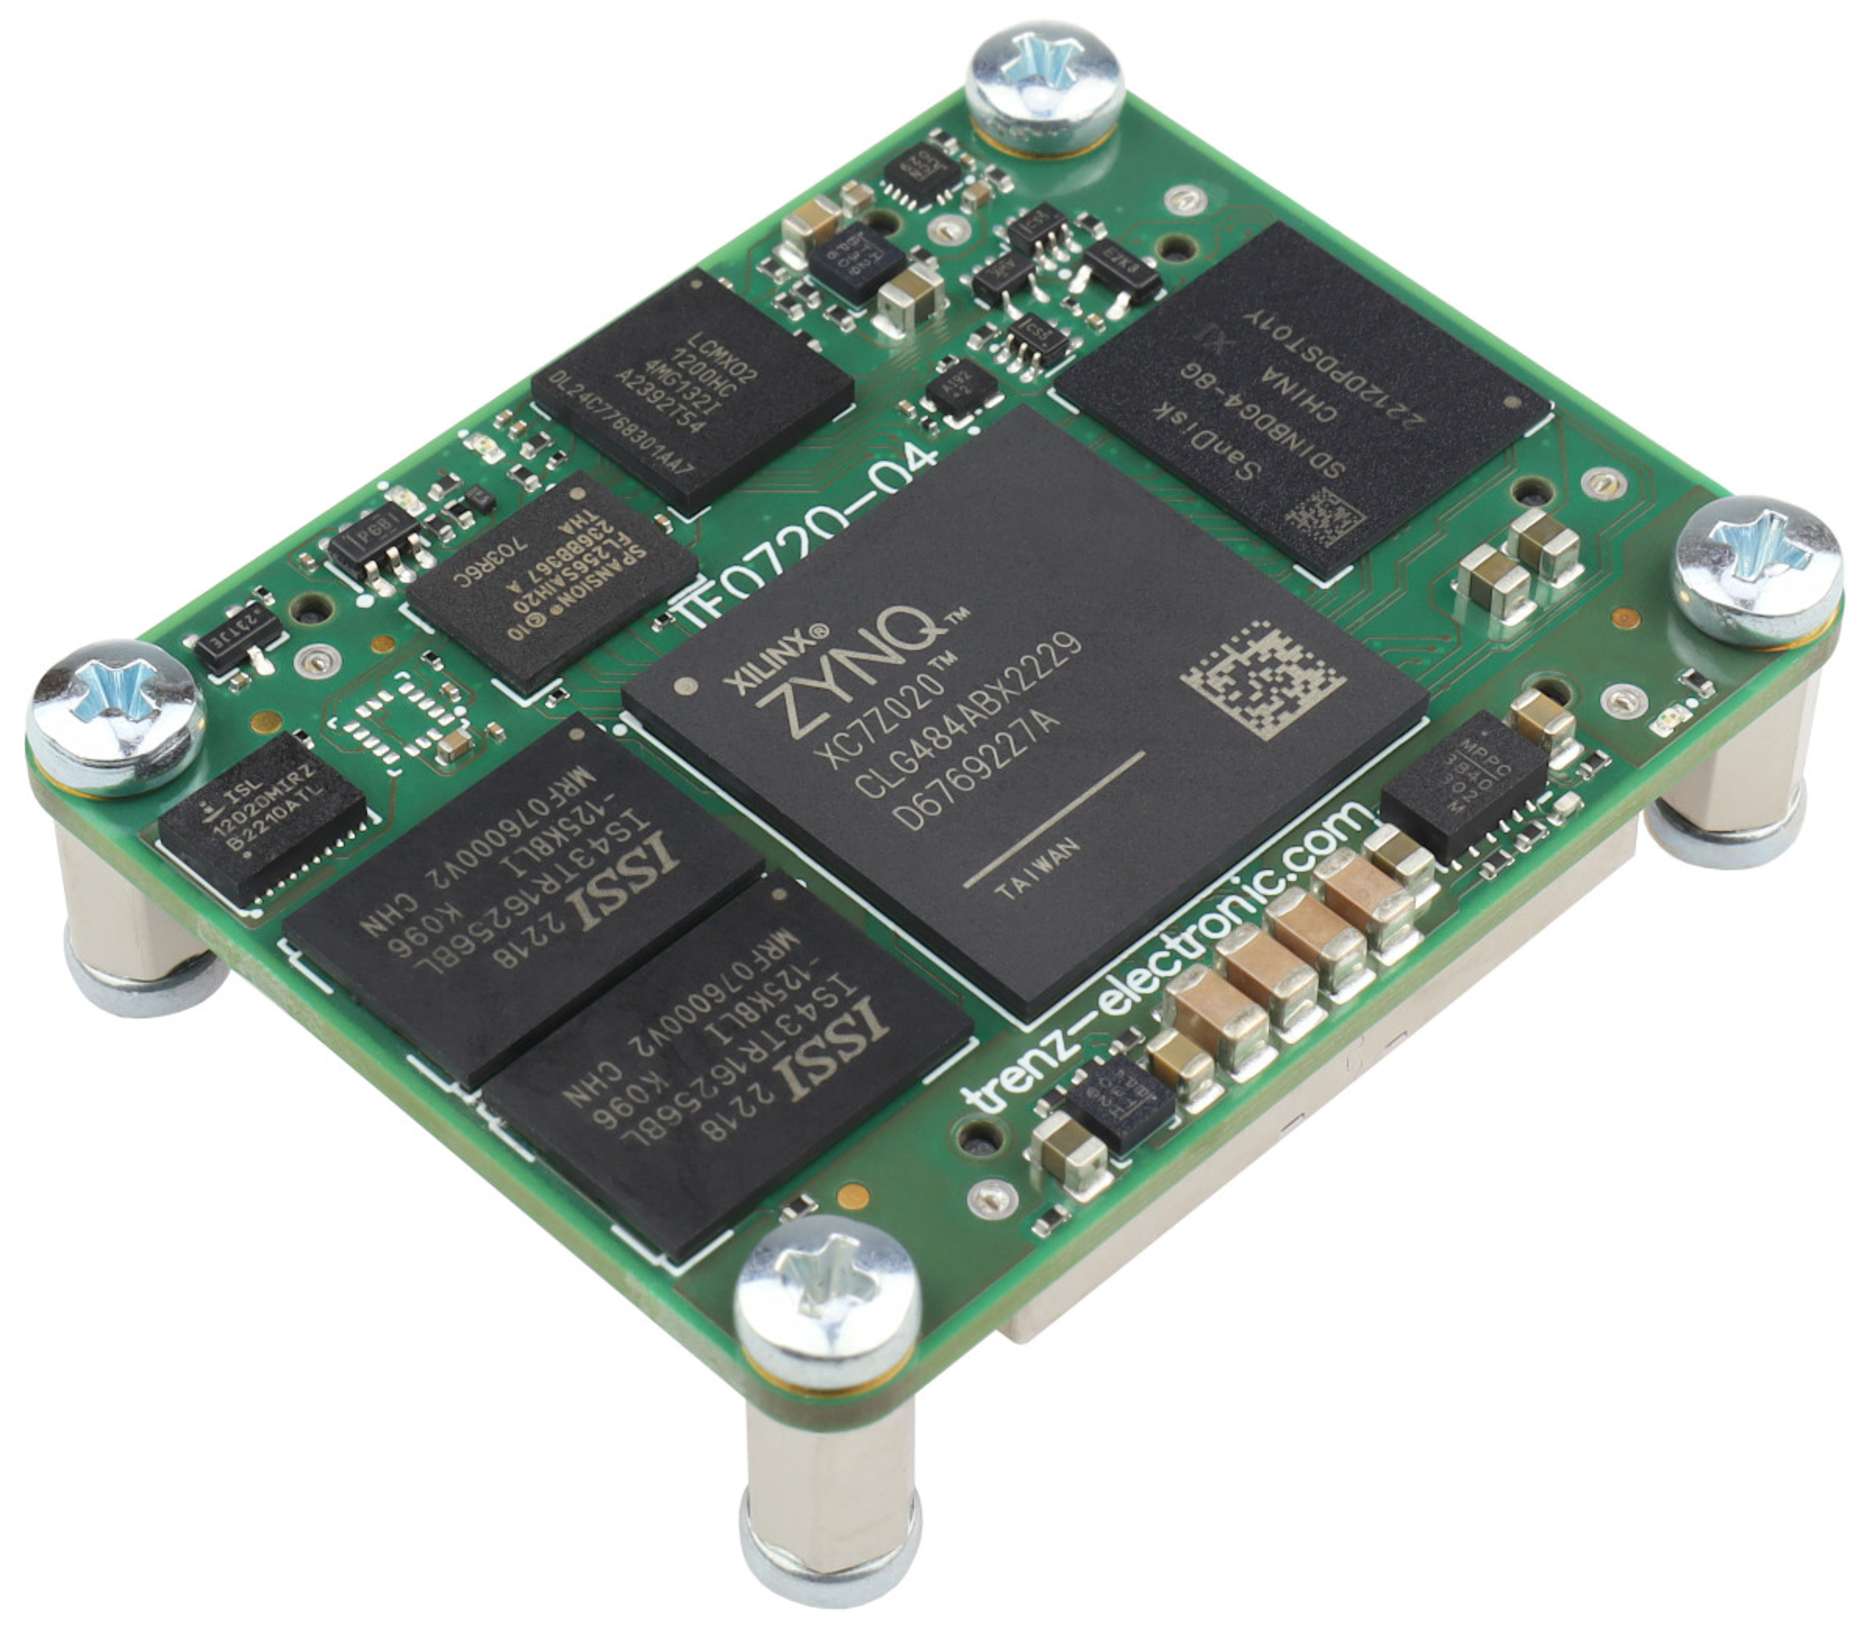
\includegraphics[width=0.6\linewidth]{sections/proc/soc.pdf}
  \caption{Trenz Electronic TE0720-04-62I33MA SoC-Module.}
  \label{fig:soc}
\end{figure}

Trenz Electronic TE0720-04-62I33MA SoC-Module features:

\begin{itemize}
    \item AMD Zynq™ XC7Z020-2CLG484I dual ARM® Cortex®-A9 MPCore™ with CoreSight™ System On Chip (SOC) IC Zynq®-7000 Artix™-7 FPGA, 85K Logic Cells 766MHz 484-CSPBGA (19x19).
    \item Rugged for high shock and vibration.
    \item 10/100/1000 tri-speed Gigabit Ethernet transceiver (PHY), SGMII accessible on a board-to-board connector.
    \item 1 GByte (32-bit) DDR3 SDRAM.
    \item 32 MByte QSPI Flash memory (for configuration and operation).
    \item 8 GByte e.MMC.
    \item Plug-on module with 2 x 100-pin and 1 x 60-pin Razor Beam High-Speed hermaphroditic Terminal/Socket Strips.
    \item 152 FPGA I/O's (75 LVDS pairs possible) and 14 MIOs available on board-to-board connectors.
    \item On-board high-efficiency DC-DC converters.
    \item Programmable through Free Vivado Standard Edition Suite.
\end{itemize}

Trenz Electronic TE0720-04-62I33MA SoC-Module is configured as: 

\begin{itemize}
    \item Low jitter clock input for sequencer and DC-DC synchronization from clock generator IC. 
    \item \SI{2.5}{\volt} external power supply for banks 13, 34 and 35. Bank 13 is not powered (unused).
    \item JTAG programming and UART communication through on board FTDI.
    \item \SI{3.3}{\volt} I2C communication through MIO pins for clock generator and EEPROM.
    \item \SI{2.5}{\volt} LVDS differential pair communication with ADC.
    \item Internal \SI{1.8}{\volt} is used for clock generator.
    \item Backplane communication through \SI{2.5}{\volt} to \SI{3.3}{\volt} voltage translator IC.
\end{itemize}